%%% Figrues
\begin{figure}
	\centering
	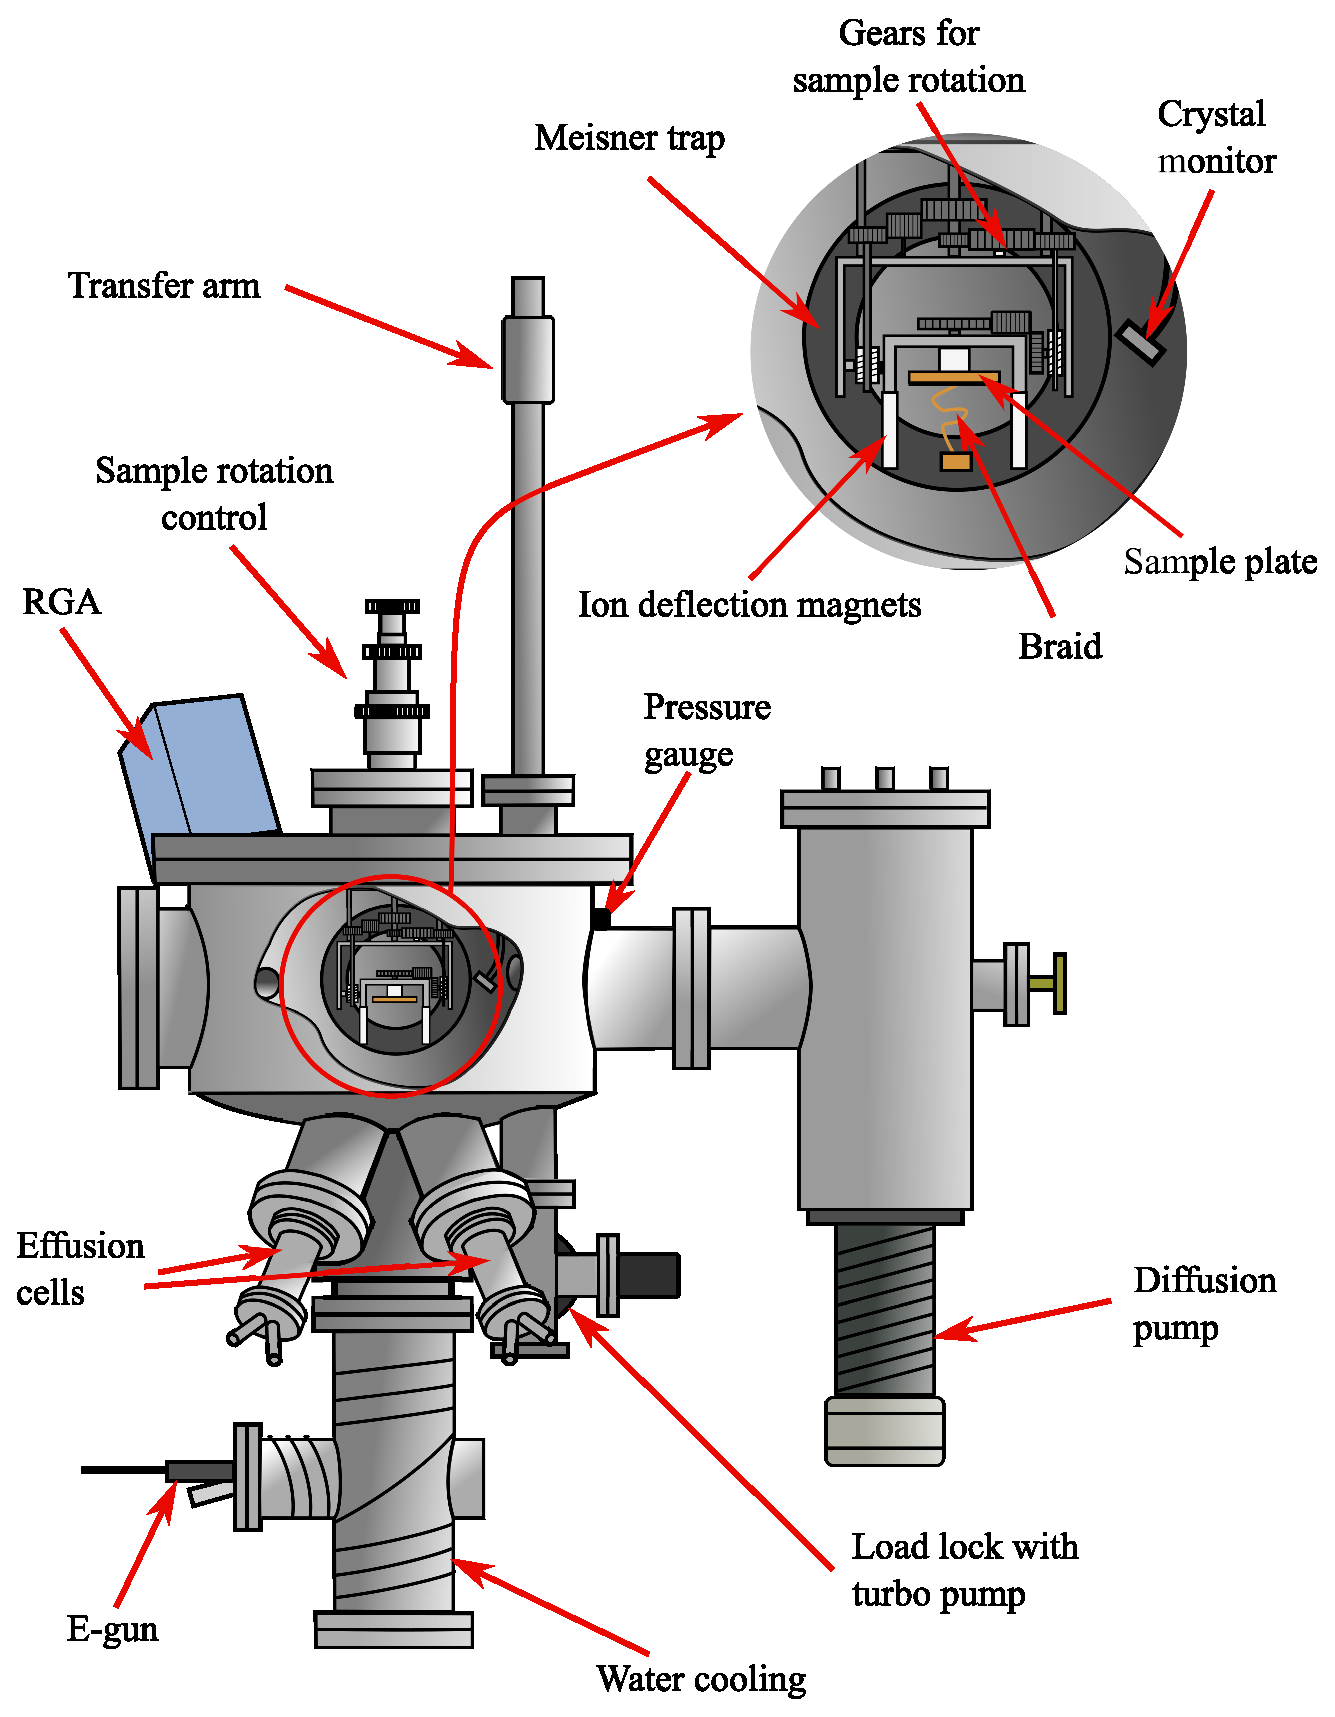
\includegraphics[width=0.5\linewidth]{slimshady_new}
	\caption{An example of how to place a figure with a caption and a lebel that you can use to cross reference the figure. Don't forget to cist the source of copied figures \cite{Batley2015} and put the label after the caption to make the cross referenced figure number correct.}
	\label{fig:fig_label}
\end{figure}

%%% Tables
\begin{table}
	\begin{center}
\begin{tabular}{ |p{3cm}||p{3cm}|p{3cm}|p{3cm}|  }
	\hline
	\multicolumn{4}{|c|}{Country List} \\
	\hline
	Country Name     or Area Name& ISO ALPHA 2 Code &ISO ALPHA 3 Code&ISO numeric Code\\
	\hline
	Afghanistan   & AF    &AFG&   004\\
	Aland Islands&   AX  & ALA   &248\\
	Albania &AL & ALB&  008\\
	Algeria    &DZ & DZA&  012\\
	American Samoa&   AS  & ASM&016\\
	Andorra& AD  & AND   &020\\
	Angola& AO  & AGO&024\\
	\hline
\end{tabular}
\caption{Tables are always a git of a pain in \LaTeXe - but here is an example table taken from \url{https://www.overleaf.com/}. Make sure the label goes after the caption for figures and tables!}
\label{tab:table_ex}
\end{center}	
\end{table}

%%% double panel and one panel with python
\begin{figure}
	\centering
	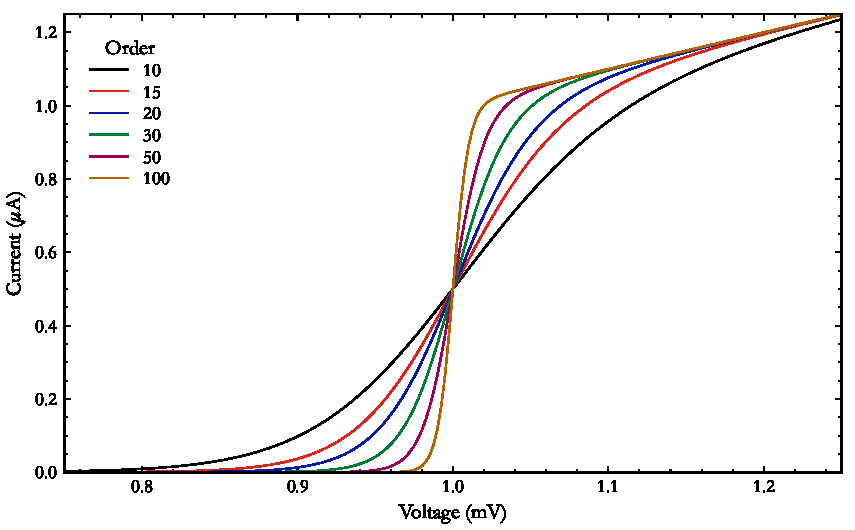
\includegraphics{fig02h_0}
	\caption{If you are making figures with Python, then I strongly recommend that you
		use the \textbf{stonerplots}\cite{stonerplots} package. It has a ``thesis'' style that is set up
		for this template.}
	\label{fig:fig_label}
\end{figure}

\begin{figure}
	\centering
	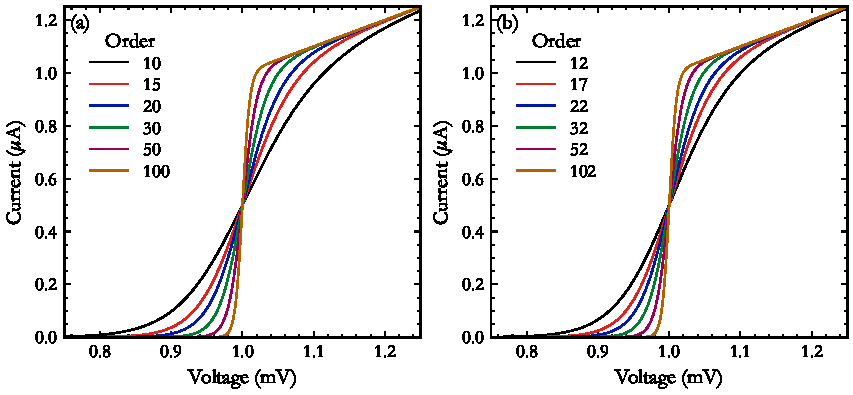
\includegraphics{fig02h_1}
	\caption{Double panel figures are also easily made with the \textbf{stonerplots}\cite{stonerplots} packae.
	and the MultiPanel context manager.}
	\label{fig:fig_label}
\end{figure}
